\documentclass{article}

\usepackage{TJU-style}

\fancyhf{}

\fancyhead[C]{电磁学实验报告}                        %用于设置页眉中间的文字   Used to set the text in the middle of the header
\fancyfoot[C]{\thepage}
% 设置页眉水平居中
\setlength{\headwidth}{\textwidth}
\fancyhfoffset[L]{\dimexpr0.5\textwidth-0.5\textwidth\relax}



\def\singlecover{
\begin{titlepage}                                               %用于单人报告的封面 For single report 
    \centering
    
\includegraphics[width=0.65\textwidth]{./images/tongji.jpg}   % 插入你的图片，调整文件名和路径 Insert your picture, adjust the file name and path
    \par\vspace{1.5cm}
    {\Large \heiti TONGJI UNIVERSITY \par} % 标题 Title
    \vspace{1cm}
    {\Huge \heiti 《电磁学实验》实验报告 \par}              % 副标题 Subtitle
    \vspace{5cm}


    % 个人信息  Personal information
    \begin{center}
        {\Large                                                 % 这里的字号也可以用别的方式修改   The font size here can also be modified in other ways
        \makebox[4em][s]{\heiti 实验名称}:\underline{\makebox[15em][c]{\heiti 锁相放大器和微弱信号测量}}\\
        \makebox[4em][s]{\heiti 学生姓名}:\underline{\makebox[15em][c]{\heiti 高雨扬}}\\
        \makebox[4em][s]{\heiti 学号}:\underline{\makebox[15em][c]{\heiti 2252146}}\\
        \makebox[4em][s]{\heiti 组号}:\underline{\makebox[15em][c]{\heiti M5}}\\
        \makebox[4em][s]{\heiti 实验日期}:\underline{\makebox[15em][c]{\heiti 2024.5.8}}\\
        }
    \end{center}

    \vfill

\end{titlepage}
}


\def\groupcover{


    \vfill
    
\end{titlepage}
}


\begin{document}
\pagenumbering{Roman}
\setcounter{page}{0}

% 切换到单人模式 Switch to single mode
\singlecover



\section*{实验目的}
1.了解数字锁相放大器的基本原理及操作,掌握利用相关性提取强噪声背景中微弱信号的原理.

2.了解锁相放大器同时测量基波和谐波成分的功能;直观观察方波的高频成分,验证方波的傅里叶展开式;了解一种采用锁相放大器测量微弱周期信号的方法.

3.掌握采用基于锁相放大技术与四线法测量微小阻抗的原理;了解LabVIEW上位机与锁相放大器之间的通信.

4.了解锁相放大器的应用;测量变容二极管内PN结电容与反偏电压的关系.

5.理解电子器件噪声的产生机制和测量原理,学会分析噪声的统计分布,了解 LabVIEW 上位机与锁相放大器的通信.


\section*{实验原理}

\subsection*{1.锁相放大器的工作原理}
锁相放大器主要由信号通道、参考通道、相敏检测器PSD和低通滤波器LPF组成.其中,信号通道的作用是对信号输入进行放大及滤波，将微弱信号放大到足以推动相敏检测器工作的电平，并且要滤除部分干扰和噪声;参考通道的作用是对参考输入进行放大或衰减，以适应相敏检测器对幅度的要求;PSD的作用是以参考通道提供的基准正弦与余弦分量作为输入，对经过信号通道放大滤波的$x(t)$进行相敏检波（乘法运算），从而实现频谱迁移过程;LPF的作用是使锁相放大器达到较大的SNIR.

\subsection*{2.强噪声背景检测弱信号实验}
本实验使用$\mu$V级别的正弦波信号，淹没在幅值可调的白噪声中，模拟客观测量环境，噪声幅值可达到目标信号的一千倍甚至一万倍。

\subsection*{3.微弱信号多谐波测量实验}
理想方波可以通过傅里叶展开为无穷多项正弦波,每一项正弦波可以视作一个级次的谐波,有原理公式$$f_{n}(t)=\frac{2E}{n\pi}\sin{(n\omega t)}$$对于目标谐波,高次谐波相当于是"噪声",因此谐波测量在本质上也是一种从噪声中提取目标信号的过程.

\subsection*{4.微小阻抗测量实验}
采用四线法,在被测元件上形成两个独立回路,分别测试被测元件两端的电压和电流.经过分析电路,阻抗测量的原理公式为$$Z_{x}=Re_{x}+Im_{x}\cdot i$$

那么对于理想纯电阻,有$$Re_{x}=R,\quad Im_{x}=0$$

对于理想纯电容,有$$Re_{x}=0,\quad Im_{x}=\frac{1}{\omega C},\quad\omega=2\pi f$$

\subsection*{5.变容二极管结电容测量实验}
势垒电容是PN结外加电压变化时,耗尽层宽度变化所等效的电容,其由多数载流子引起.而扩散电容仅由少数载流子引起,反向偏置时可以忽略.

根据讲义中原理图示,有原理公式$$C_{X}=\frac{V_{out}}{V_{sine}-V_{out}}\times C_{0}$$式中各量意义在讲义中已经给出.

\subsection*{6.电阻热噪声测量实验}
可以认为,载流子微观热运动的随机涨落体现在宏观效应上便是电阻热噪声的根源.热力学温度$T$下,阻值为$R$的电阻的实际开路噪声电压为$$U=\sqrt{4kTRB}$$

通过锁相放大器,可以测量得到电阻热噪声和放大器底噪的叠加,通过短接合适的电阻消除放大器底噪,可以测得电阻热噪声电压.

\section*{实验内容}
在不同的具体实验中,根据实验讲义的指导,输出合适的波形信号,根据原理图连接实验线路,调节对应电学量,记录所需的数据和图像,并进行分析得出结论.



\section*{实验仪器}
OE1022E锁相放大器,教学实验仪,示波器,若干BNC信号线;微弱信号教学实验仪;已安装LabVIEW程序的电脑,四线法夹具,若干电阻电容器件;变容二极管;已安装BNC连接头的电阻器.

\section*{数据记录处理}
本次实验中,完成强噪声背景检测弱信号实验,微弱信号多谐波测量实验,变容二极管结电容测量实验共三项实验内容.

\subsection*{1.强噪声背景检测弱信号实验}

第一组因设备原因无法达到$V_{in}=1000$mVrms的条件,因而同时减弱正弦波信号和噪声背景大小至讲义中参考数据的$\frac{1}{10}$,之后调节合适的噪声信号大小来实现实验要求的信噪比.此外,第一组和第五组的实验图像遗漏记录.

其余组均正常记录数据和截图.数据和仪器截图如下.


    \captionof{table}{强噪声背景第一组}        % 使用captionof命令来实现表格标题 Use the captionof command to achieve the table title
    \label{tab:tab1}
    \begin{tabular}{c|c|c|c|c} 
		\hline
        $V_{in}$幅值/mVrms & 噪声信号/mVrms & 信噪比 & 锁相放大器R值/mVrms & 示波器测量值/mVrms \\ 
        \hline
        100 & 10 & 20dB & 101.6 & 101.3 \\ 
        \hline 
    \end{tabular}

    \captionof{table}{强噪声背景第二组}        % 使用captionof命令来实现表格标题 Use the captionof command to achieve the table title
    \label{tab:tab1}
    \begin{tabular}{c|c|c|c|c} 
		\hline
        $V_{in}$幅值/mVrms & 噪声信号/mVrms & 信噪比 & 锁相放大器R值/mVrms & 示波器测量值/mVrms \\ 
        \hline
        100 & 100 & 0dB & 102.4 & 140.3 \\ 
        \hline
    \end{tabular}

	\begin{minipage}[c]{1.0\textwidth}
		\centering
		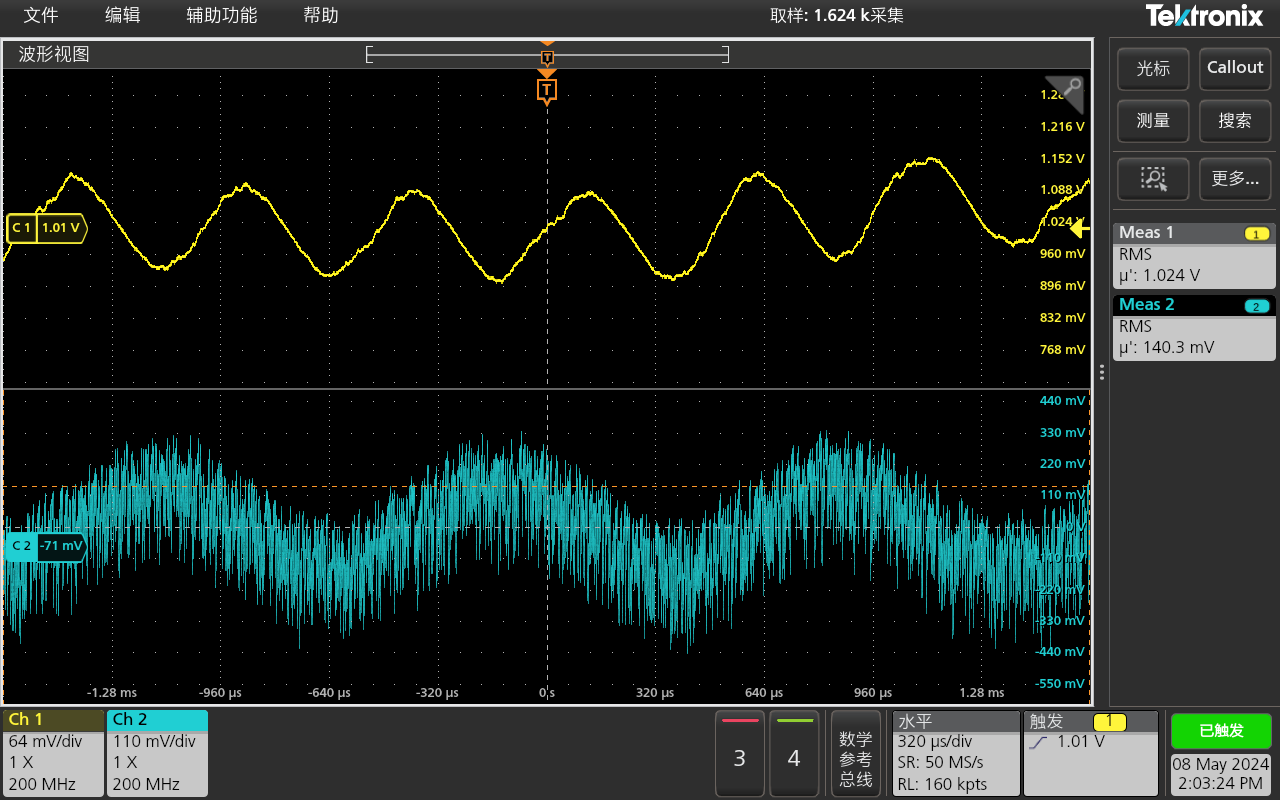
\includegraphics[width=0.9\textwidth]{images/1.png}
		\caption*{图1:强噪声背景第二组截图}
	\end{minipage}


    \captionof{table}{强噪声背景第三组}        % 使用captionof命令来实现表格标题 Use the captionof command to achieve the table title
    \label{tab:tab1}
    \begin{tabular}{c|c|c|c|c} 
		\hline
        $V_{in}$幅值/mVrms & 噪声信号/mVrms & 信噪比 & 锁相放大器R值/mVrms & 示波器测量值/mVrms \\ 
        \hline
        10 & 100 & -20dB & 10.29 & 99.41 \\ 
        \hline
    \end{tabular}

	\begin{minipage}[c]{1.0\textwidth}
		\centering
		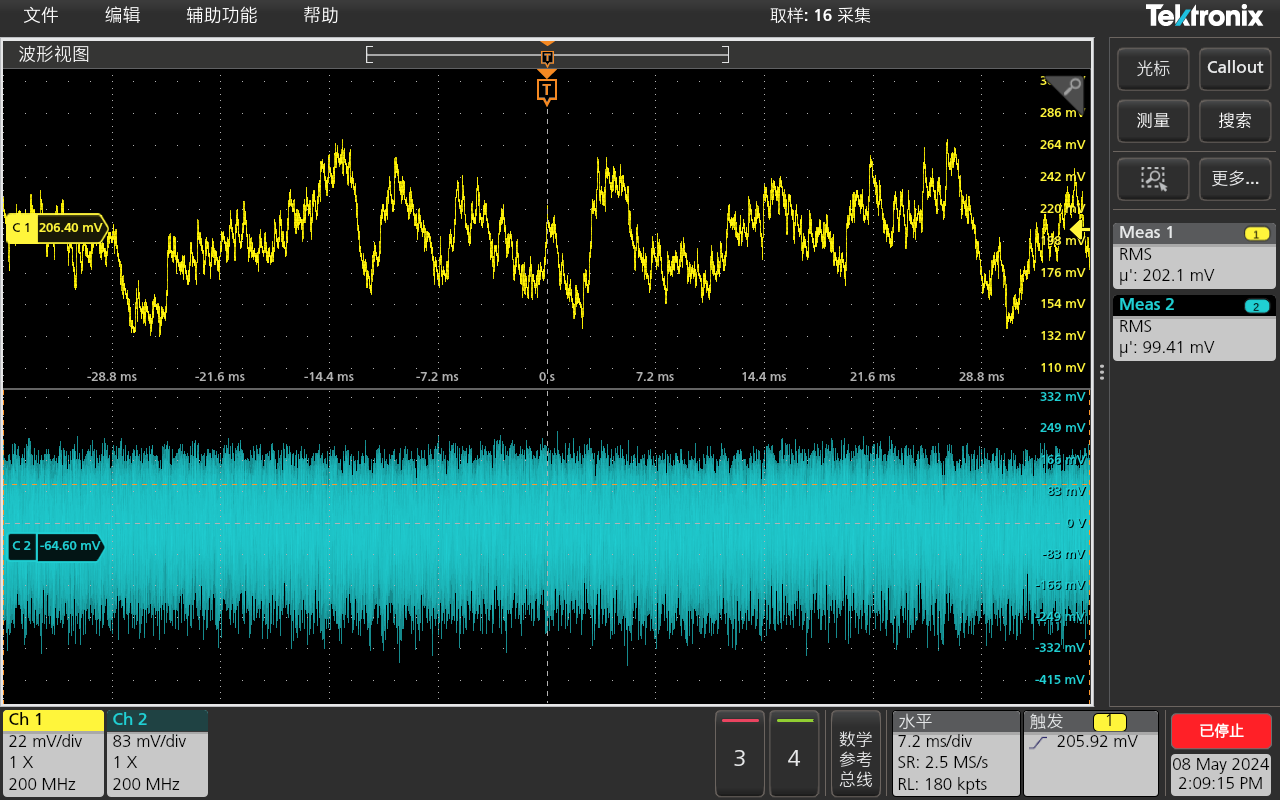
\includegraphics[width=0.9\textwidth]{images/2.png}
		\caption*{图2:强噪声背景第三组截图}
	\end{minipage}


    \captionof{table}{强噪声背景第四组}        % 使用captionof命令来实现表格标题 Use the captionof command to achieve the table title
    \label{tab:tab1}
    \begin{tabular}{c|c|c|c|c} 
		\hline
        $V_{in}$幅值/mVrms & 噪声信号/mVrms & 信噪比 & 锁相放大器R值/mVrms & 示波器测量值/mVrms \\ 
        \hline
        1 & 100 & -40dB & 1.37 & 98.55 \\ 
        \hline
        
    \end{tabular}

	\begin{minipage}[c]{1.0\textwidth}
		\centering
		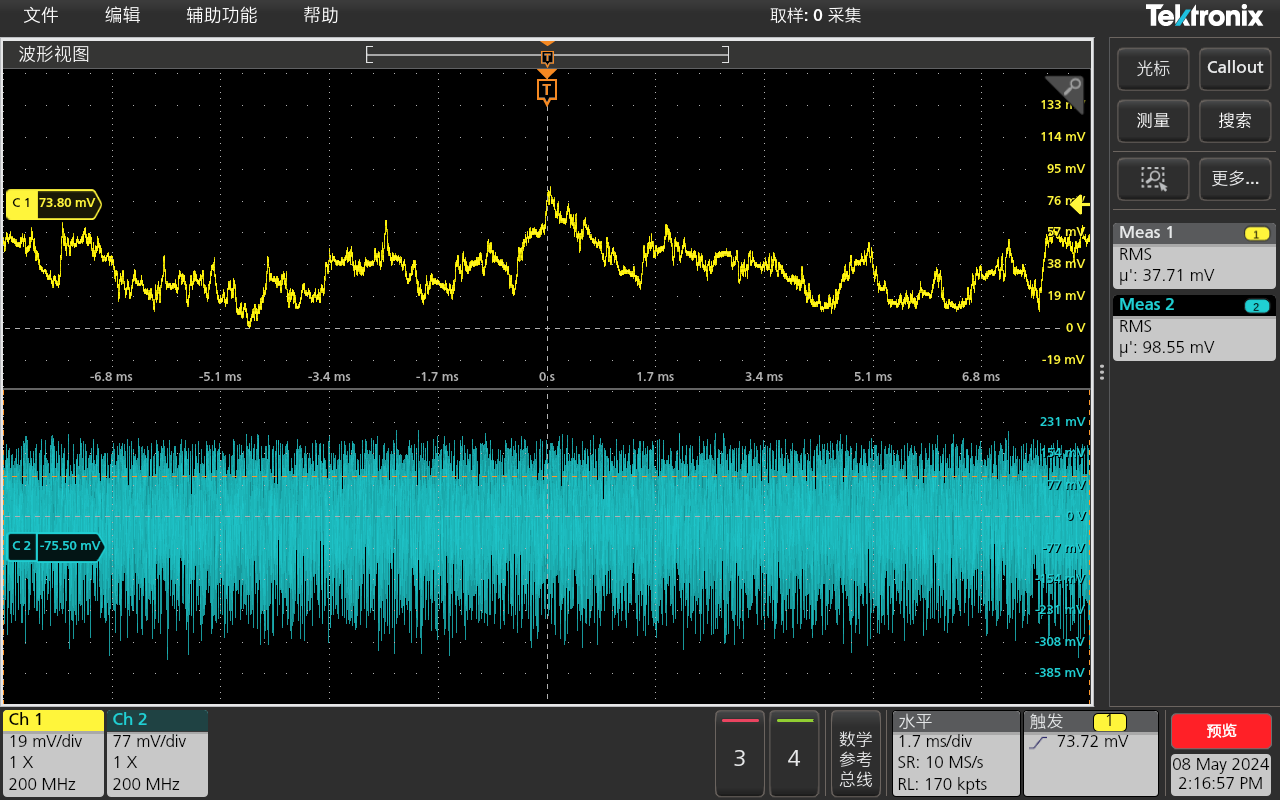
\includegraphics[width=0.9\textwidth]{images/3.png}
		\caption*{图3:强噪声背景第四组截图}
	\end{minipage}


    \captionof{table}{强噪声背景第五组}        % 使用captionof命令来实现表格标题 Use the captionof command to achieve the table title
    \label{tab:tab1}
    \begin{tabular}{c|c|c|c|c} 
		\hline
        $V_{in}$幅值/mVrms & 噪声信号/mVrms & 信噪比 & 锁相放大器R值/mVrms & 示波器测量值/mVrms \\ 
        \hline
        0.1 & 100 & -60dB & 0.704 & 100.6 \\
        \hline
        
    \end{tabular}


\subsection*{2.微弱信号多谐波测量实验}

这部分实验数据和计算后的误差记录如下.

\centering
\captionof{table}{强微弱信号多谐波测量}        % 使用captionof命令来实现表格标题 Use the captionof command to achieve the table title
\label{tab:tab1}
\begin{tabular}{c|c|c|c} 
	\hline
	谐波奇次项 & 理论计算值$\mu$Vrms & 锁相放大器测量值mVrms & 误差  \\ 
	\hline
	1 & 225.113 & 235.65 & 4.68\% \\
	\hline
	3 & 75.038 & 78.47 & 4.57\% \\
	\hline
	5 & 45.023 & 46.97 & 4.32\% \\
	\hline
	7 & 32.159 & 46.97 & 4.23\% \\
	\hline
	9 & 25.013 & 26.13 & 4.47\% \\
	\hline
	11 & 20.465 & 21.46 & 4.86\% \\
	\hline
	13 & 17.316 & 18.21 & 5.16\% \\
	\hline
	
\end{tabular}

\raggedright

\subsection*{3.变容二极管结电容测量实验}
实验中,设置了锁相放大器的参数"Ref.frequency"即测量频率为10.000kHz.

原始数据进行计算后记录如下,同附Excel拟合的关系图.

\clearpage
\centering
\captionof{table}{变容二极管结电容测量}        % 使用captionof命令来实现表格标题 Use the captionof command to achieve the table title
\label{tab:tab1}
\begin{tabular}{c|c|c|c|c|c} 
	\hline
	反偏电压/V & 实验测得R值/$\mu$V & 电容值/nF & 反偏电压/V & 实验测得R值/$\mu$V & 电容值/nF \\ 
	\hline
	1.0 & 274.05 & 0.192 & 4.6 & 67.35 & 0.046 \\
	\hline
	1.2 & 253.27 & 0.170 & 4.8 & 62.49 & 0.042 \\
	\hline
	1.4 & 234.47 & 0.160 & 5.0 & 58.35 & 0.040 \\
	\hline
	1.6 & 217.75 & 0.151 & 5.2 & 52.38 & 0.036 \\
	\hline
	1.8 & 203.43 & 0.141 & 5.4 & 47.24 & 0.032 \\
	\hline
	2.0 & 187.35 & 0.130 & 5.6 & 42.25 & 0.029 \\
	\hline
	2.2 & 173.39 & 0.120 & 5.8 & 37.96 & 0.026 \\
	\hline
	2.4 & 159.53 & 0.110 & 6.0 & 34.61 & 0.024 \\
	\hline
	2.6 & 148.27 & 0.102 & 6.2 & 31.99 & 0.022 \\
	\hline
	2.8 & 135.91 & 0.094 & 6.4 & 30.04 & 0.020 \\
	\hline
	3.0 & 125.35 & 0.086 & 6.6 & 28.26 & 0.019 \\
	\hline
	3.2 & 115.19 & 0.079 & 6.8 & 27.21 & 0.018 \\
	\hline
	3.4 & 106.43 & 0.073 & 7.0 & 26.03 & 0.018 \\
	\hline
	3.6 & 98.37 & 0.068 & 7.2 & 25.25 & 0.017 \\
	\hline
	3.8 & 91.20 & 0.063 & 7.4 & 24.43 & 0.017 \\
	\hline
	4.0 & 85.38 & 0.059 & 7.6 & 23.71 & 0.016 \\
	\hline
	4.2 & 78.57 & 0.054 & 7.8 & 23.23 & 0.016 \\
	\hline
	4.4 & 74.34 & 0.051 & 7.9 & 22.93 & 0.015 \\
	\hline	
\end{tabular}
\raggedright


\begin{minipage}[c]{1.0\textwidth}
	\centering
	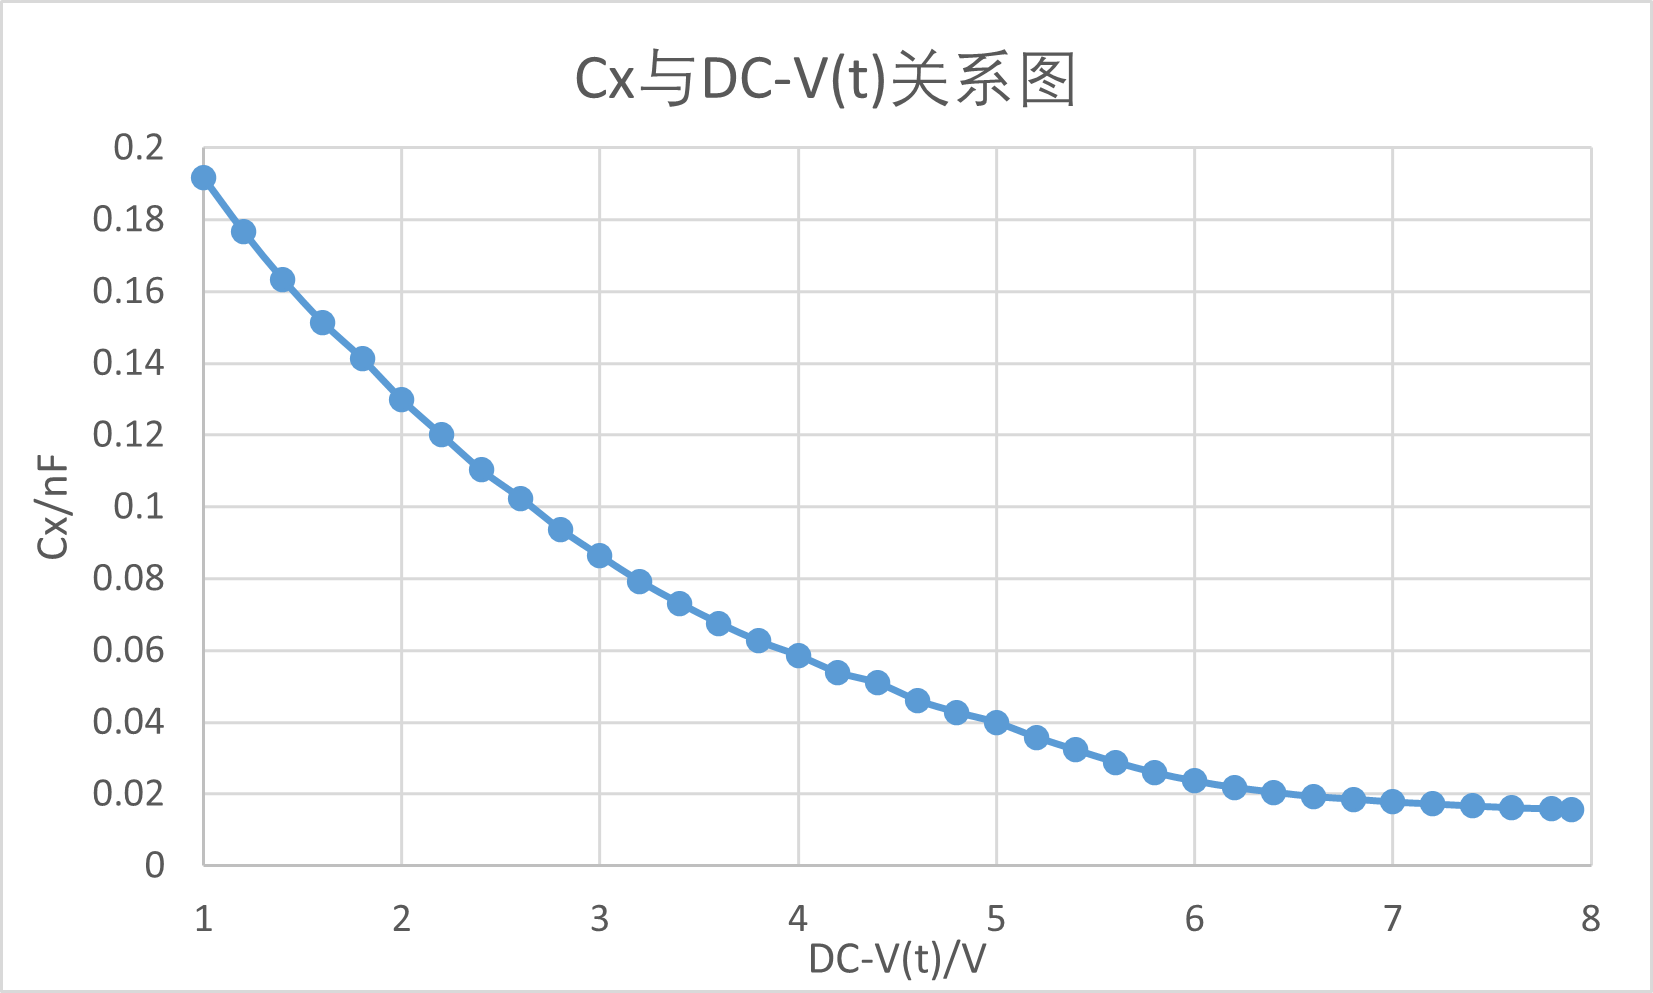
\includegraphics[width=0.9\textwidth]{images/4.png}
	\caption*{图4:$C_{x}$与$DC-V(t)$关系图}
\end{minipage}


\section*{讨论与分析}

\subsection*{思考题}
\subsubsection*{强噪声背景检测弱信号实验思考题}
1.在不同信噪比情况下,采用同样的时间常数及陡降,观察输出被测信号的$R$值及$\theta$值,发现什么规律？

    在较高的信噪比情况下,系统对信号的测量更加准确,因此输出的$R$值会更接近信号的真实值.相位测量往往比幅度测量更容易受到噪声的干扰,因此在低信噪比情况下,相位$\theta$的稳定性可能会受到更大的影响,导致测量结果的波动更大.

2. 同一信噪比情况下,调整滤波器时间常数及陡降,观察输出信号的$R$值及$\theta$值,发现什么规律?

    较小的时间常数通常会导致更快的响应速度,使系统能够更快地跟踪信号的变化,从而得到更接近真实值的$R$值和$\theta$值.

    较小的陡降通常意味着更快的信号衰减率,使系统能够更快地对信号进行衰减,从而得到更接近真实值的$R$值;然而陡降对$\theta$的稳定性和准确性会有间接影响,通过影响系统本身而体现.

\subsubsection*{微弱信号多谐波实验思考题}
1.500$\mu$V的方波信号可以用实验室通用的示波器测试到吗?

本组实验未测得该方波信号,但可以测得衰减前的5V信号,如下图.
\begin{minipage}[c]{1.0\textwidth}
	\centering
	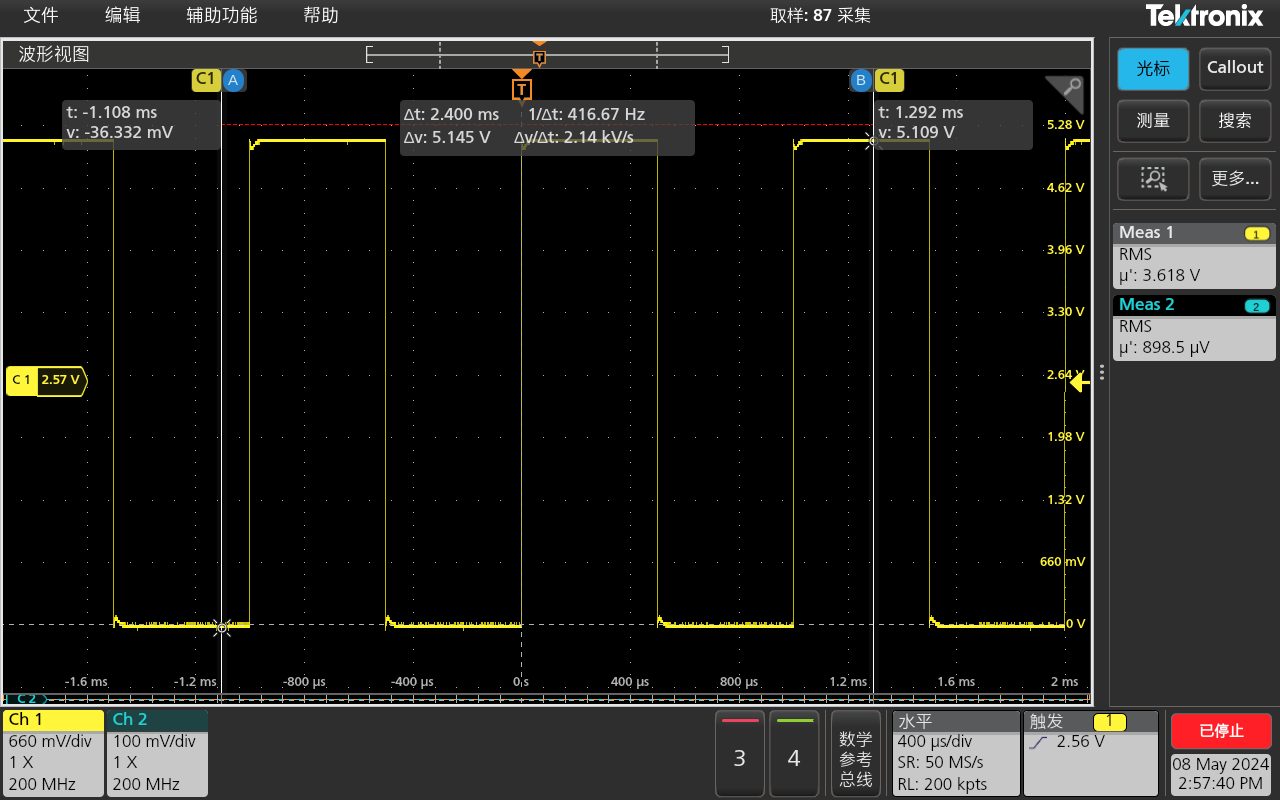
\includegraphics[width=0.9\textwidth]{images/5.png}
	\caption*{图5:方波信号检验图}
\end{minipage}

2.怎样用实验的方法测量微小三角波,锯齿波等周期信号?

更换合适的信号发生器产生所需的三角波或锯齿波信号,选取并调整好合适的示波器来观察波形,以及测量信号的参数.

3.本实验的多谐波测量实验能够适用任意周期信号吗?

事先对信号的周期性特征进行评估并得到良好结果的前提下,能够适用;不然,对于周期过长或特征不明显的信号,不一定能够得到实验结果.

\subsubsection*{变容二极管结电容测量实验思考题}
1.参考本方法,思考三极管和场效应管的寄生电容或者电感如何测量.

三极管的寄生电容可以使用频率响应测试等方法来测量Miller电容,场效应管的寄生电容可以通过使用频率响应测试来测量栅极-源极电容;两者的寄生电感都可以使用LRC测试仪器,或者网络分析仪来测量串联寄生电感的值.

2.某些传感器的阻抗在外界环境情况下会随环境快速响应,例如测量发动机气缸的温度的变化.这种情况可以考虑用一个热敏电阻(电阻值随着温度变化而变化)作为传感器,由于发动机气缸的温度变化很快,因此传统的方法测量信噪比低.思考及设计采用锁相放大技术进行测量的方案.

选择具有高性能的锁相放大器,能够在高频率下快速准确地跟踪信号变化;将热敏电阻作为传感器,连接到锁相放大器的输入端;在放大器的输入端可以添加信号调理电路,例如滤波器,以滤除高频噪声和干扰信号;将锁相放大器输出的信号连接到数据采集系统,以记录和分析温度传感器的变化.

\section*{实验结论}

本次实验习得了锁相放大器的使用方法,以及利用锁相放大器测量部分类型信号得到了合理的实验结果,验证了实验原理中的公式.

\clearpage
\section*{原始数据单}
\begin{minipage}[c]{1.0\textwidth}
	\centering
	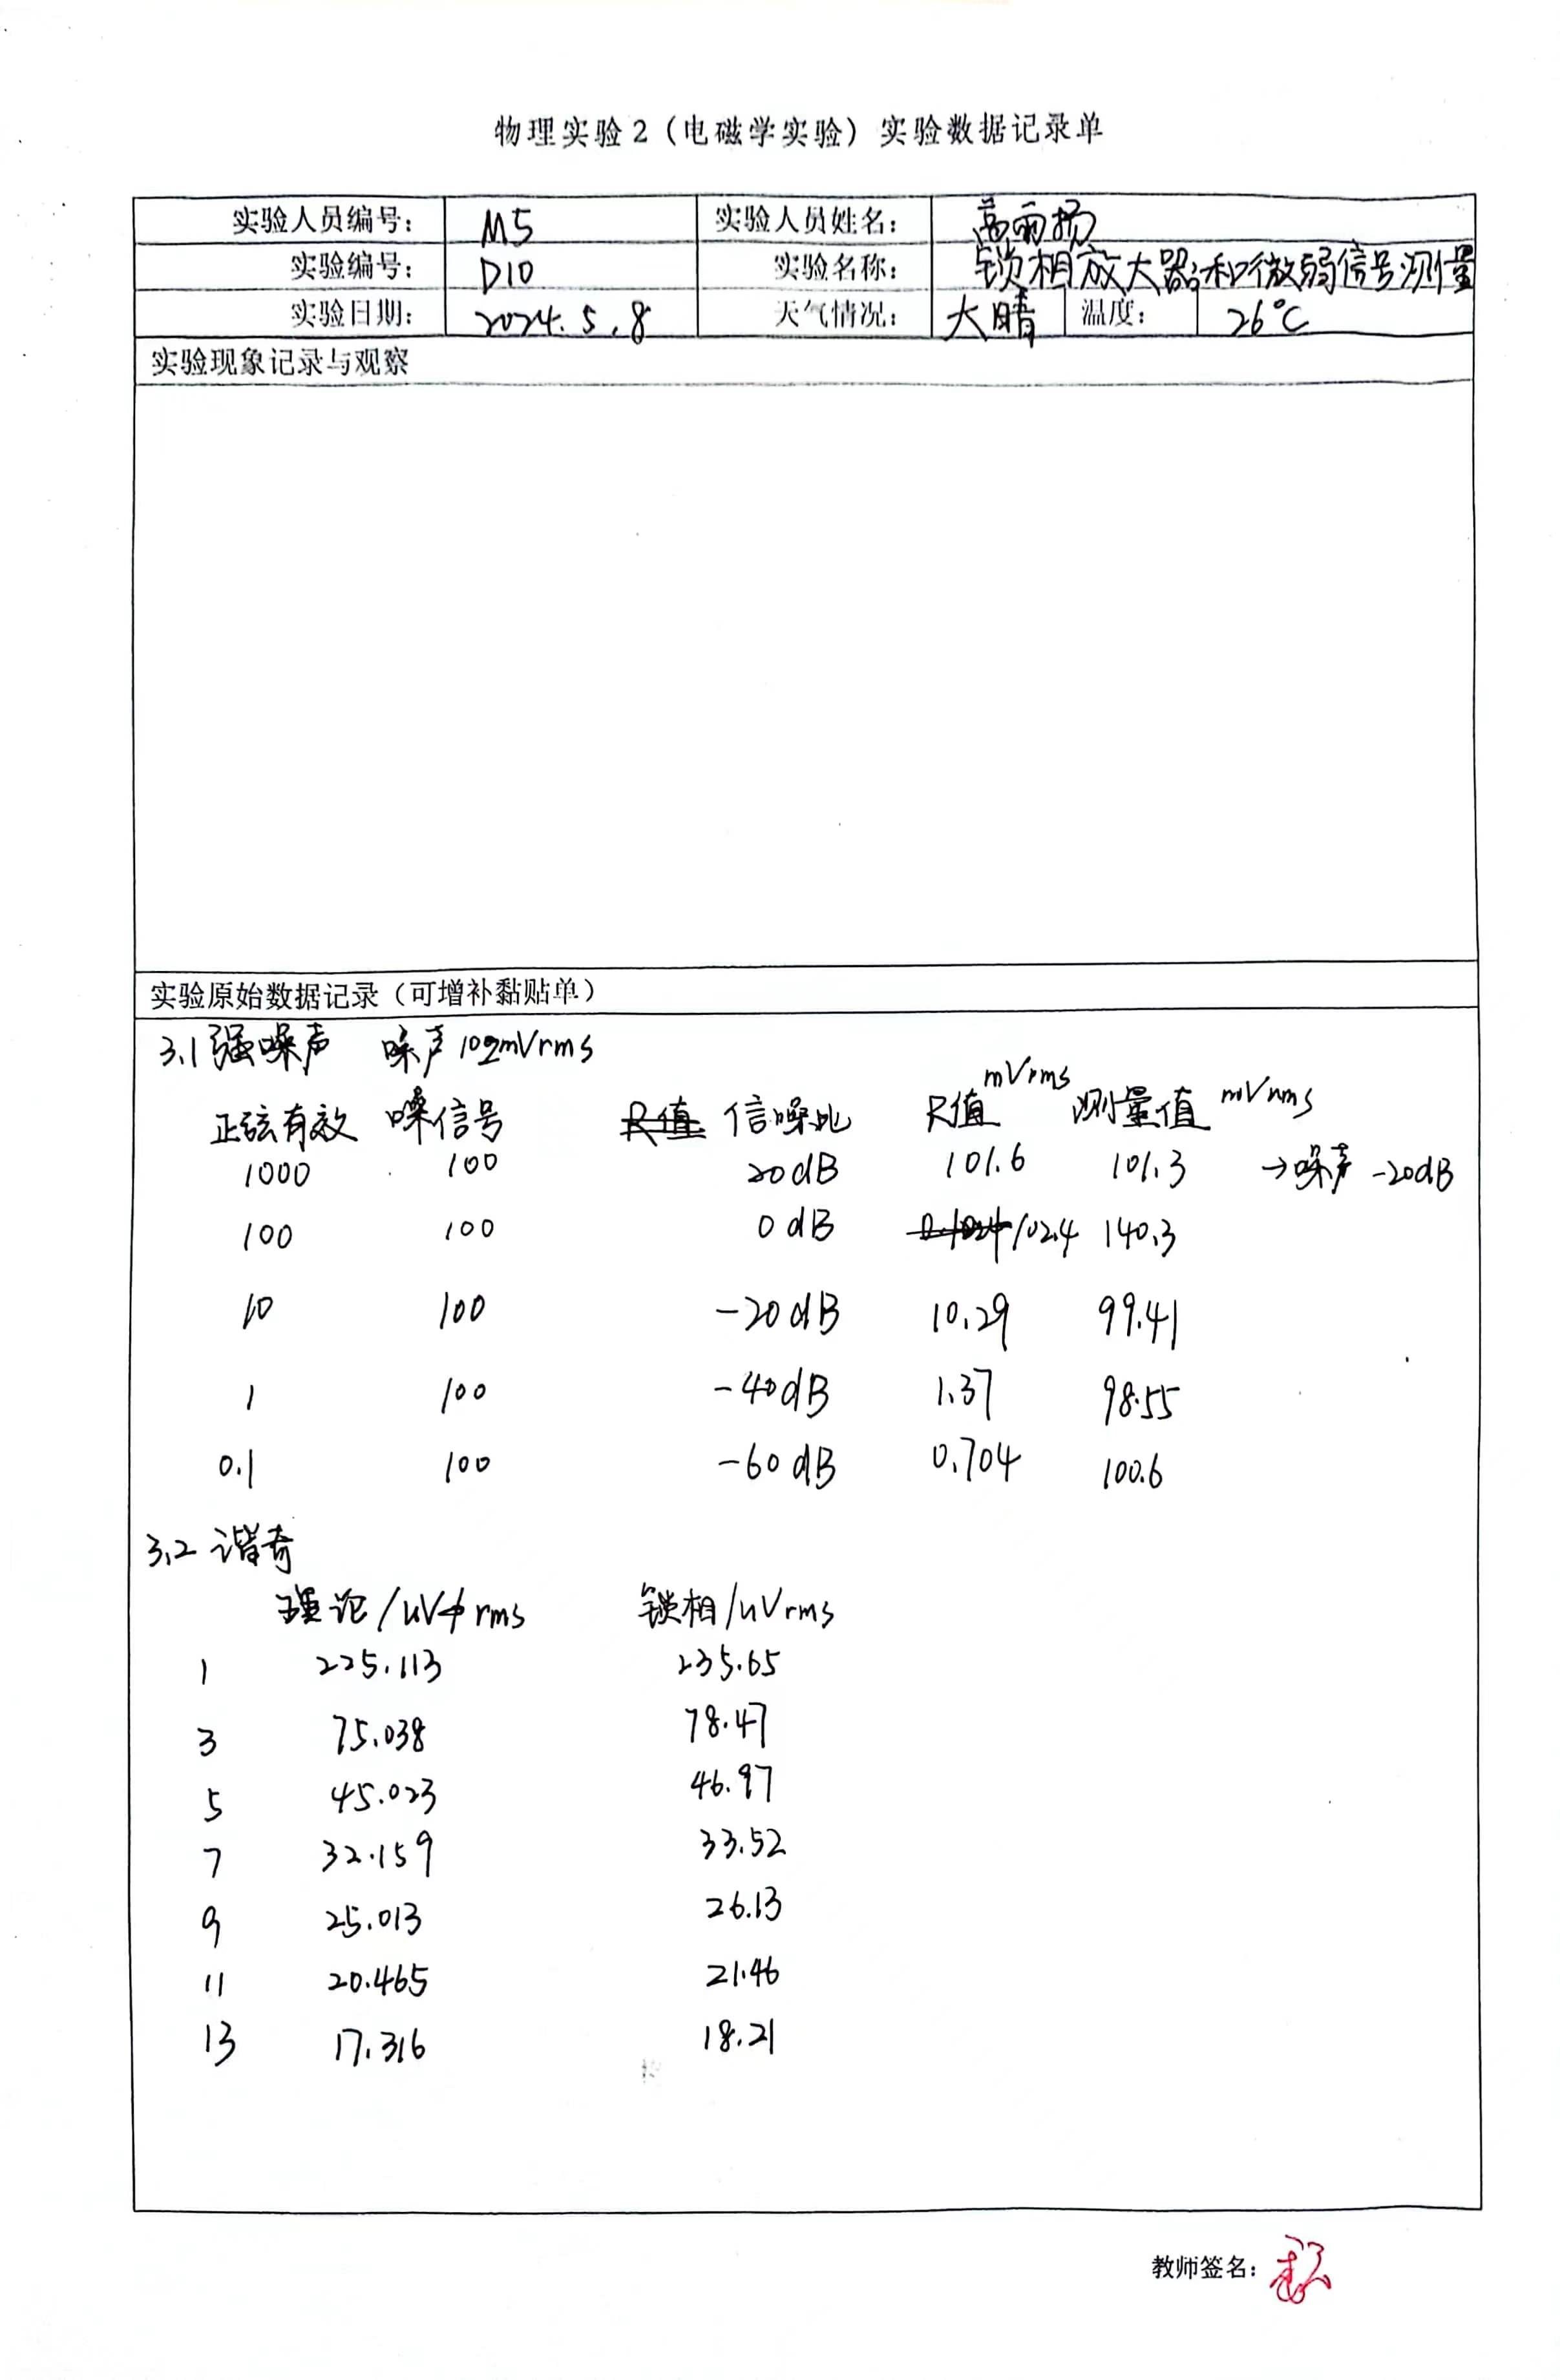
\includegraphics[width=0.9\textwidth]{images/2.jpg}
	\caption*{图6:数据单(正面)}
\end{minipage}

\clearpage
\begin{minipage}[c]{1.0\textwidth}
	\centering
	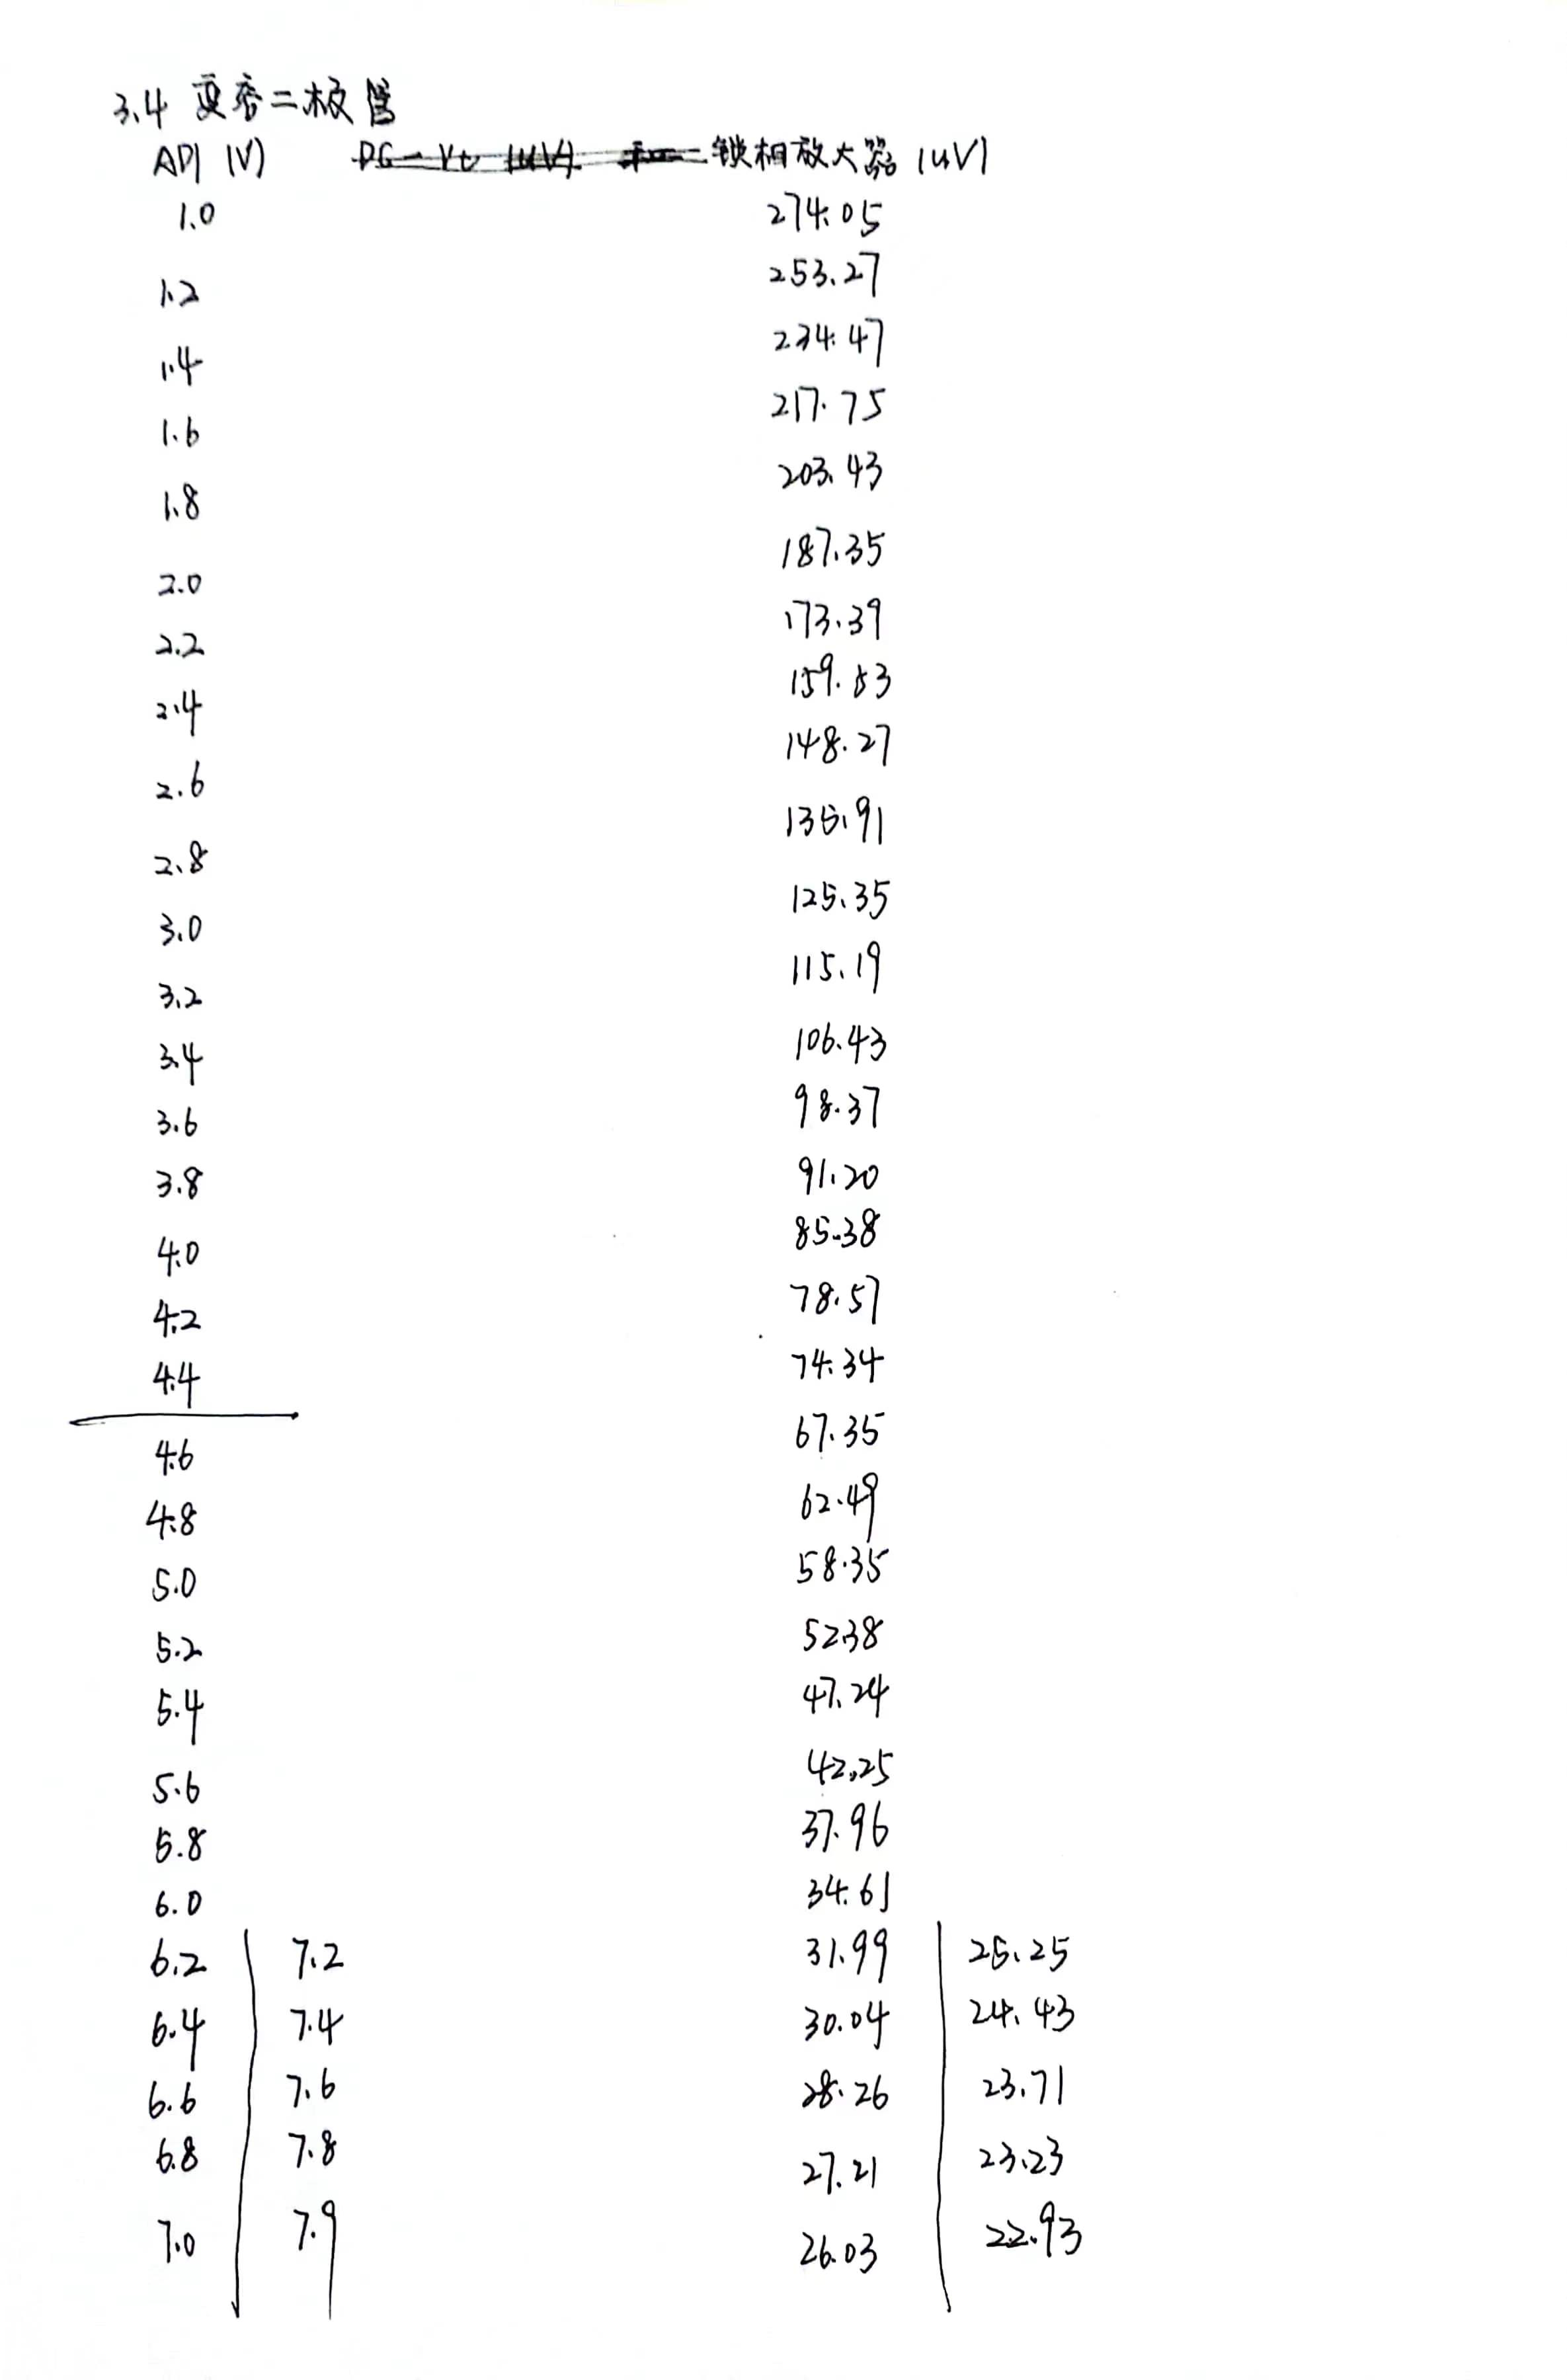
\includegraphics[width=0.9\textwidth]{images/1.jpg}
	\caption*{图7:数据单(反面)}
\end{minipage}

\end{document}
